\chapter{Description du travail réalisé}
\label{chap:description}

Pour réaliser ce projet, nous avons décidé de créer plusieurs structures de données afin de représenter le problème et de le résoudre, représentées par des classes dans le langage C++.

\section{Donnée "Ile"}
Notre structure de donnée Ile contient plusieurs informations:
\begin{itemize}
    \item son degré
    \item sa coordonnée en abscisse dans la grille
    \item sa coordonnée en ordonnée dans la grille
    \item le nombre de ponts reliés à cette île
    \item un tableau d'îles qui représente les voisins possibles
    \item un tableau d'îles représentant les voisins réels
    \item un booléen qui sera vrai si l'île est résolue, faux sinon
\end{itemize}
\smallbreak
Pour finir, nous avons aussi ajouté deux attributs à notre structure Ile concernant les composantes connexes. Nous avons décidé de les représenter comme des arbres: on désigne une île comme étant "chef" de sa composante connexe, et toutes les autres îles de cette composante seront "fils" (directs ou non, cependant il est préférable qu'ils soient directs pour la suite) de celui-ci. Les deux attributs à ce sujet sont donc la hauteur de l'arbre représentant la composante connexe à laquelle l'île appartient, ainsi qu'un pointeur vers une autre île de la composante connexe qui sera son père direct dans l'arbre.
\smallbreak
En ce qui concerne les méthodes de cette classe, la grande majorité ne changera que l'île concernée (accesseurs) et une seule interagit avec un autre objet: DéjàVoisin. Son but est de vérifier si l'île dans laquelle est appelée la méthode est déjà reliée à celle passée en paramètre (autrement dit si elle fait partie des voisins réels). Cette méthode renvoie un booléen.

\section{Donnée "Pont"}
Notre structure de donnée Pont ne contient que peu d'informations:
\begin{itemize}
    \item un pointeur vers la première île
    \item un pointeur vers la deuxième île
    \item le "nombre" de ponts (simple ou double)
    \item un booléen vrai si le pont est vertical, faux sinon
\end{itemize}
\smallbreak
Concernant le nombre de ponts, celui-ci sera égal à un s'il n'existe qu'un seul pont entre les deux îles, ou égal à deux s'il en existe deux. Dans notre vision des choses, deux ponts entre les mêmes îles sera considéré comme un seul objet Pont avec son attribut "nombre" ègal à deux plutôt que deux objets Pont distincts l'un de l'autre.

\section{Donnée "IleOuPont"}
Après avoir créé deux structures de donnée, Ile et Pont, nous avons fait le choix d'en créer une regroupant, en quelque sorte, ces deux dernières. En effet, les deux seuls attributs présents dans IleOuPont sont deux informations concernant le fait de savoir s'il s'agit d'une île ou bien d'un pont, comme nous aurions pu le deviner au vu du nom de cette dernière. Par conséquent, il existe dans cette classe, un attribut se trouvant être un pointeur de Ile et un attribut se trouvant être un pointeur de Pont. De plus, elle contient, en plus des attributs précédemment cités :
\begin{itemize}
    \item Trois constructeurs de classe différents afin de déclarer un objet de ce type de plusieurs manières avec notamment le constructeur par défaut, le constructeur où l'on passe en paramètre un pointeur de type Ile et le constructeur où l'on passe en paramètre un pointeur de type Pont.
    \item Deux accesseurs en écriture afin d'opérer directement un changement sur une ile ou sur un pont.
    \item Deux accesseurs en lecture afin pouvoir récupérer l'île ou le pont présent 
\end{itemize}
\smallbreak
Cette structure de donnée fut créée dans un but précis qui était celui de vouloir créer un vecteur à deux dimensions des îles ou des ponts présents dans la grille. Ainsi chaque case, représentée par des coordonnées en abscisse et en ordonnée, comportait une donnée de type IleOuPont. Afin de savoir s'il s'agissait d'une île ou d'un pont, cette dernière, comme expliqué précédemment, comporte deux attributs servant à le déterminer. S'il s'avérait être un pont alors le pointeur sur Ile serait NULL et inversement ce serait le pointeur sur Pont qui serait NULL. Nous pouvons très bien aussi n'avoir ni de pont ni d'île dans cette case auquel cas les deux attributs seraient NULL mais dans tous les cas, nous ne pouvons avoir les deux attributs non NULL en même temps.

\section{Donnée "Grille"}
Dans cette dernière partie de ce chapitre, nous allons aborder un point important qui est celui de la classe Grille. Elle ne comporte pas moins de sept attributs la complétant :
\begin{itemize}
    \item Un entier signé représentant la hauteur max de la grille de jeu
    \item Un entier signé représentant la longueur max de la grille de jeu
    \item Le vecteur à deux dimensions des îles ou des ponts dans la grille précédemment évoqué
    \item Un booléen signalant si toutes les îles sont résolues
    \item Un entier représentant le nombre de composantes connexes 
    \item Un entier représentant le nombre d'îles présentes
    \item Un entier représentant le nombre d'îles devenues résolues
\end{itemize}
\smallbreak
Tout d'abord il est bon de savoir , avant de commencer quelconque approfondissement, que nous introduisons un fichier texte lors de la compilation de notre programme contenant des informations essentielles sur la grille de jeu. En effet, ce dernier contient notamment la hauteur max et la longueur max de la grille présents dans les attributs de notre classe. Ainsi, nous récupérons ces données à l'aide d'une des méthodes présentes dans Grille, la méthode "lecture", qui elle même va en appeler d'autres afin de procéder à la construction de la grille à partir du fichier texte. Cette méthode va, dans un premier temps, récupérer la hauteur et la longueur max pour ensuite y initialiser la grille et pour finir en y rajoutant les îles dans celle-ci. Effectivement, nous pouvons aussi trouver dans le fichier texte les coordonnées en abscisse et en ordonnée de chacune des îles présentes ainsi que leur valeur, permettant ainsi leur placement. \newline
Ensuite, c'est aussi dans cette classe que nous allons trouver la méthode d'affichage. Cette dernière nous permet donc d'avoir un aperçu concret de notre jeu avec les différentes îles représentées par leur valeur reliées par des ponts simples ou doubles, verticaux ou horizontaux symbolisés par des traits tels que "--", "==", "|" ou encore "||". \newline
De surcroît, nous avons bien évidemment, différents accesseurs en lecture et en écriture concernant tous nos attributs précédemment cités. Plus précisément, nous pouvons par exemple, grâce à "getUneIleOuUnPont", accéder à ce que contient une case précise dans le vecteur à deux dimensions à l'aide de coordonnées. De même pour "setUneIleOuUnPont" où il s'agit, ici, de remplir une case par une île ou un pont de la classe IleOuPont.  \newline
Concernant la notion de composante connexe présente dans la classe Grille, nous nous assurons simplement de savoir combien de composante connexes reste-il afin de déterminer si nous pouvons considérer la grille comme résolu. Pour ce faire, nous vérifions si nous obtenons qu'une seule composante connexe et nous vérifions aussi si toutes les îles sont résolues, et si c'est le cas, alors la grille l'est aussi. Quand à la méthode "unionComposantesConnexes" prenant deux pointeurs de Ile en paramètre, elle a pour but d'unifier les deux composantes connexes de ces îles, qui sont reliées entre elles par un pont, en leur inscrivant, ce qu'on a appelé, le même chef qui n'est autre qu'une île père de toutes les autres îles dans sa composante. \newline
Pour finir, nous avons aussi écrit des méthodes ayant trait aux voisins des îles avec notamment "RecupVoisinsPossibles" nous permettant de récupérer les voisins de notre île sur lesquels il est possible d'y relier au moins un pont. Cette dernière est complétée, en quelque sorte, par "majVoisinsReels" qui va être appelée lorsque nous allons créer un pont afin d'effectuer une mise à jour de tous les voisins de toutes les îles. De ce fait, nous avons trois méthodes principales liées entre elles, "tracerPont" qui va appeler "reglesPonts" lorsque nous tombons sur une île dans la grille. Ensuite, "reglesPonts" va vérifier les règles précédemment expliquées et va donc appeler (notamment) "creerPont" lorsque nous entrerons dans une de ces règles. Et pour terminer, "creerPont" déterminera la nature du pont afin que celui-ci puisse être affiché et effectuera donc la mise à jour des voisins réels. Ces dernières méthodes sont essentielles quand au fonctionnement de notre résolveur.





\section{Fichier "Main"}
Lorsque l'on appelle notre résolveur dans un terminal, un fichier texte doit être passé en paramètre dans lequel est inscrit la taille de la grille (sa largeur et sa hauteur), ainsi que toutes les îles sous la forme "x y degré". Une fois appelé, le résolveur va, dans le main, extraire du fichier les informations avec les méthodes prévues à cet effet. Ensuite, nous ferons une première traversée entière de la grille afin d'initialiser les voisins possibles de toutes les îles (méthode RecupVoisinsPossibles). Nous continuons en faisant appel à la méthode tracerPonts de grille. Une fois la grille résolue, on affiche dans le terminal la solution trouvée. \newline

\begin{figure}[htp]
  \centering
  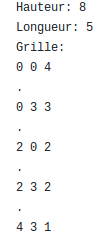
\includegraphics[width=2.35cm]{images/FichierTexte}
  \caption{Fichier texte passé en paramètre}
\end{figure}
